\thispagestyle{lichsutoanhocnone}
\pagestyle{lichsutoanhoc}
\graphicspath{{../lichsutoanhoc/pic/}}
\everymath{\color{lichsutoanhoc}}
\blfootnote{$^1$\color{lichsutoanhoc}Cộng tác viên Viện Toán học.}
\begingroup
\AddToShipoutPicture*{\put(0,616){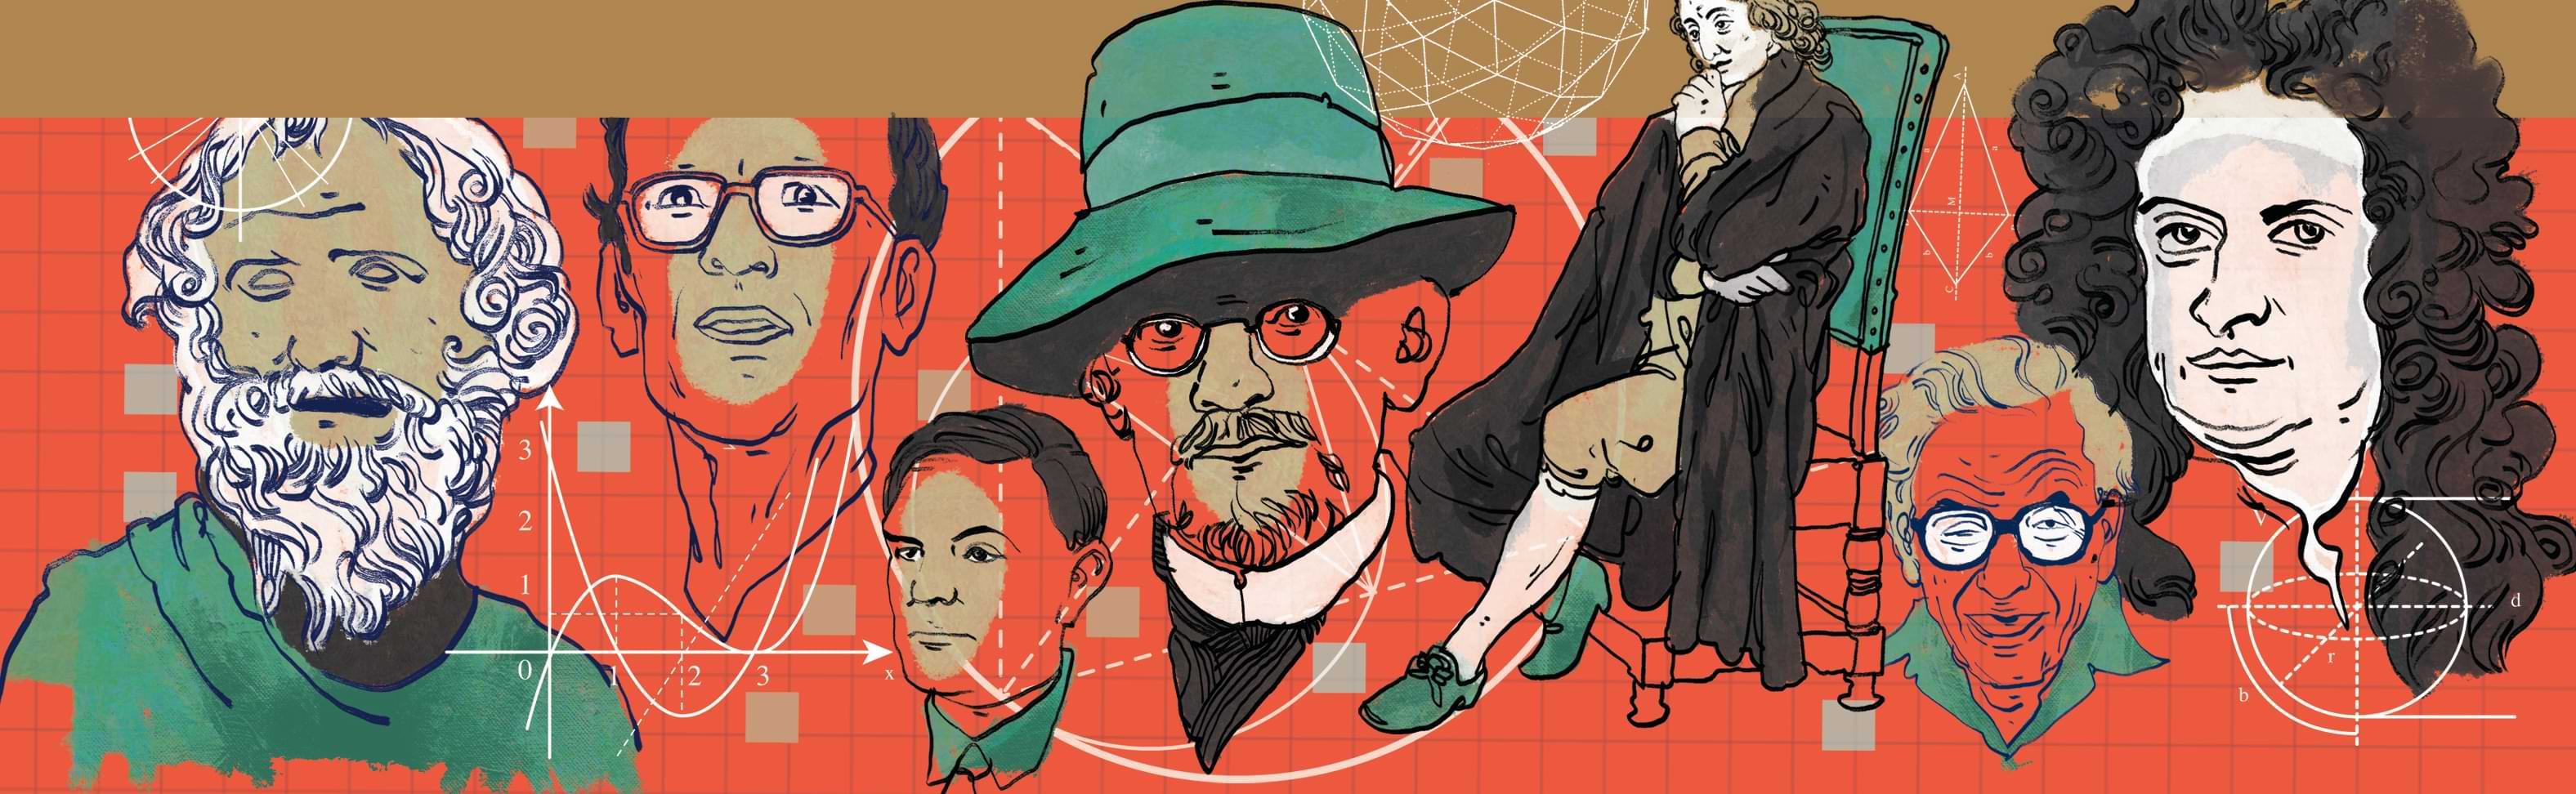
\includegraphics[width=19.3cm]{../bannerlichsu}}}
\AddToShipoutPicture*{\put(58,466){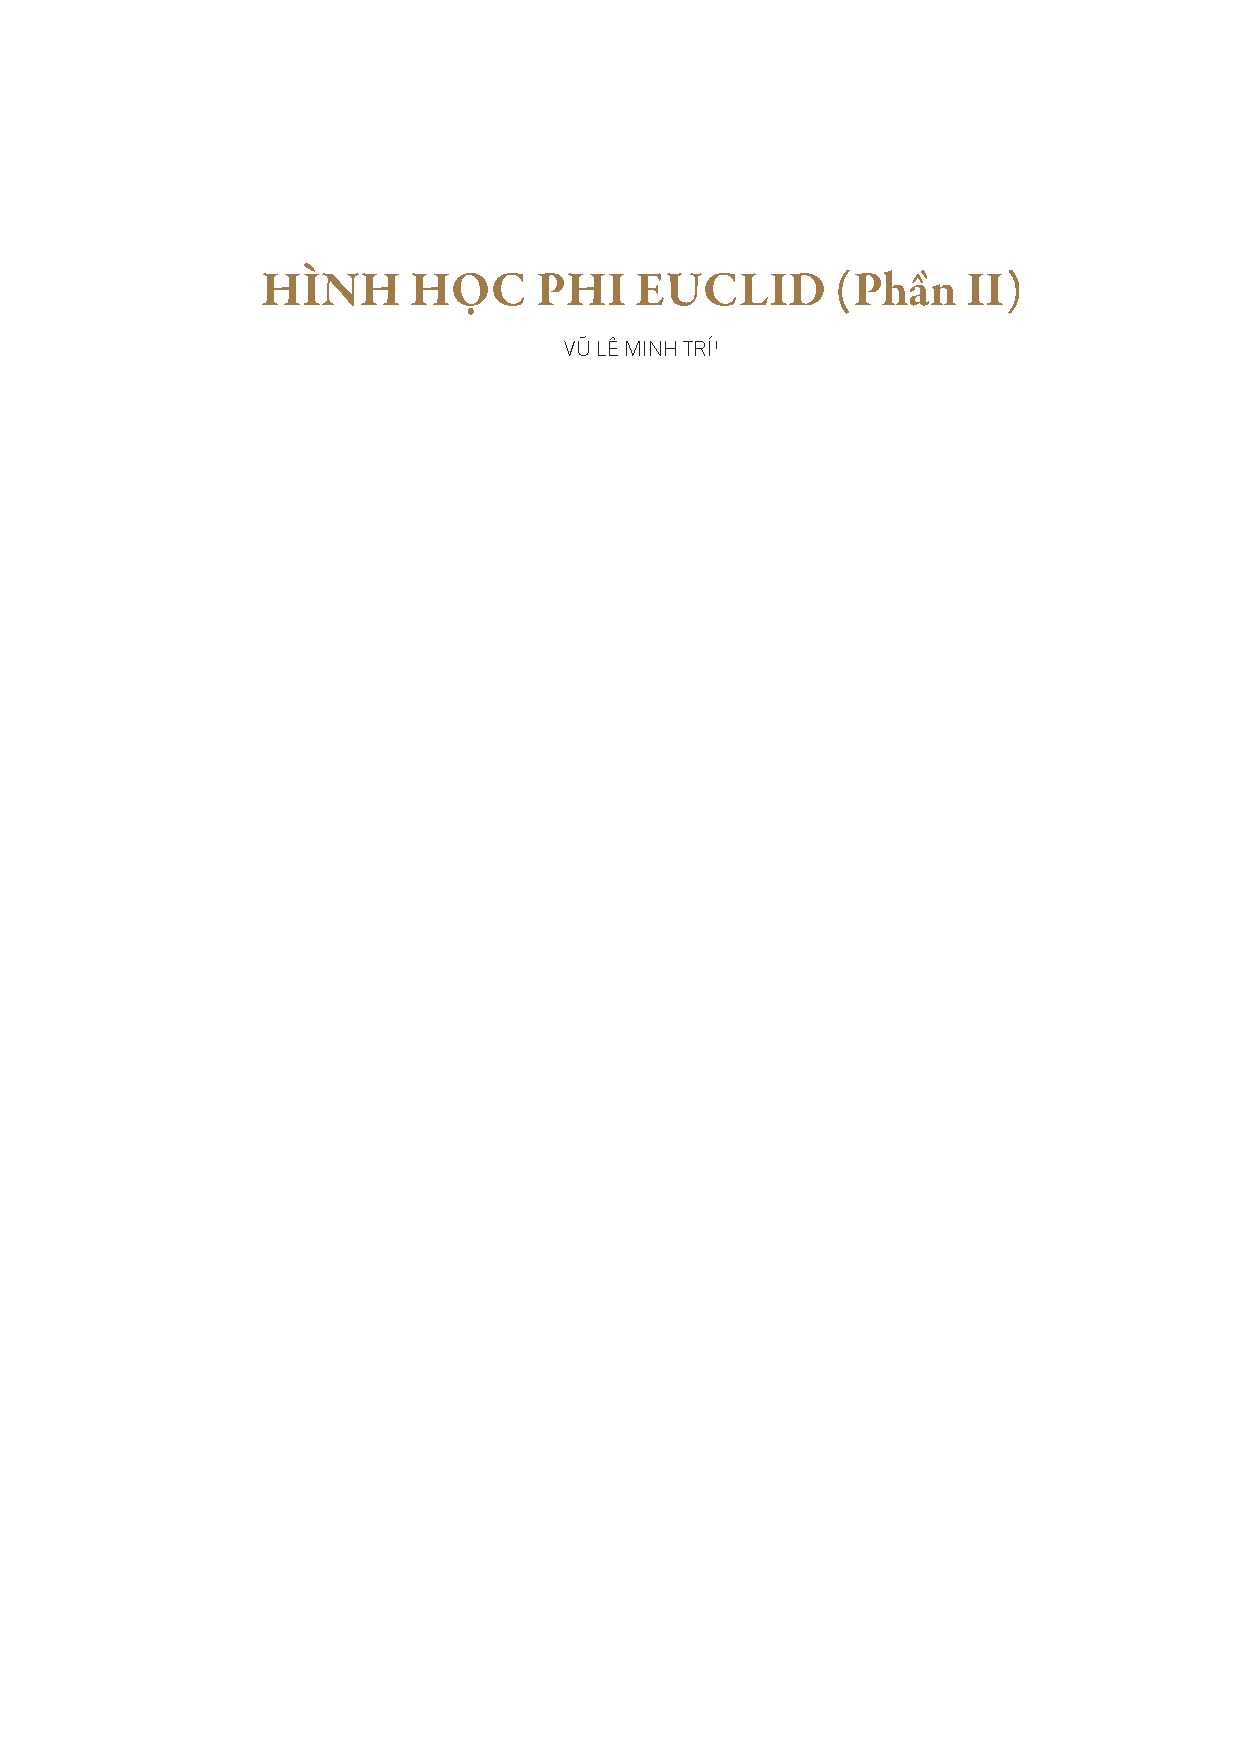
\includegraphics[scale=1]{../tieude3.pdf}}}
\centering
\endgroup

\vspace*{240pt}

\begin{multicols}{2}
	\textbf{\color{lichsutoanhoc}Học viện Plato}
		\vskip 0.1cm
		Thế kỷ thứ tư TCN đã mở đầu bằng cái chết của Socrates (khoảng $470-399$ TCN), một học giả đã áp dụng phương pháp biện chứng của Zeno và bác bỏ thuyết Pythagoras của Archytas (khoảng $420-347$ TCN). Socrates thừa nhận rằng khi còn trẻ, ông đã bị thu hút bởi những câu hỏi như tại sao tổng $2 + 2$ lại bằng tích $2 \times 2$  nhưng khi nhận ra rằng cả toán học và khoa học đều không thể thỏa mãn mong muốn của ông để  hiểu bản chất của sự vật, ông đã tự nghiên cứu để hiểu những điều bản chất.
		\vskip 0.1cm
		Trong \textit{Phaedo} của Plato, cuộc đối thoại trong đó những giờ cuối cùng của Socrates được mô tả rất đẹp, chúng ta thấy những nghi ngờ siêu hình sâu sắc như thế nào loại trừ mối quan tâm của Socrate về toán học hoặc khoa học tự nhiên:
		\vskip 0.1cm
		\textit{Tôi không thể tự thỏa mãn bản thân rằng, khi một cái được thêm vào một cái, mà phép cộng được thực hiện trở thành hai. 
		\vskip 0.1cm
		Tôi không thể hiểu làm thế nào khi tách khỏi nhau, mỗi trong số chúng là một chứ không phải hai, và bây giờ, khi chúng được kết hợp lại với nhau, chỉ là sự đặt cạnh nhau, là nguyên nhân khiến chúng trở thành hai.}
		\vskip 0.1cm
		Do đó, ảnh hưởng của Socrates trong sự phát triển của toán học là không đáng kể, nếu không nói là tiêu cực. Điều đáng ngạc nhiên là chính học trò và người ngưỡng mộ ông là Plato đã trở thành cảm hứng toán học của thế kỷ thứ tư TCN. 
		\vskip 0.1cm
		Mặc dù bản thân Plato không có đóng góp kết quả toán học nổi bật cụ thể nào, nhưng ông đã là trung tâm của hoạt động toán học thời gian đó, hướng dẫn và truyền cảm hứng cho sự phát triển của toán học. Tại cửa trường học của ông, Học viện (The Academy) ở Athens, được khắc khẩu hiệu ``Ai không biết hình học không vào đây".
		\begin{tBox}
			ΑΓΕΩΜΕΤΡΗΤΟΣ ΜΗΔΕΙΣ ΕΙΣΙΤΩ.
		\end{tBox}
		Sự nhiệt tình của Plato đối với toán học khiến ông được biết đến không phải với tư cách là một nhà toán học, mà là ``người tạo ra các nhà toán học".
			\end{multicols}
	\begin{figure}[H]
	\vspace*{5pt}
	\centering
	\captionsetup{labelformat= empty, justification=centering}
	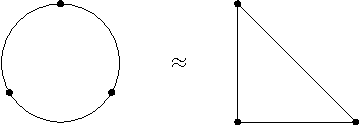
\includegraphics[width= 1\linewidth]{H7}
	\caption{\small\textit{\color{lichsutoanhoc}Hình $6$: The School of Athens của Rafael tại Vaticant.}}
	\vspace*{-10pt}
\end{figure}
\begin{multicols}{2}
%		\vskip 0.1cm
		Sáu nhà toán học (ngoài Plato và Aristotle) sống giữa năm mất của Socrates ($399$ TCN) và năm mất của Aristotle ($322$ TCN) -- gồm Theodorus xứ Cyrene (thế kỷ V TCN), Theaetetus (khoảng $414-369$ TCN), Eudoxus xứ Cnidus (khoảng $410-347$ TCN), hai anh em Menaechmus ($380-320$ TCN) và Dinostratus ($390-320$  TCN), và Autolycus xứ Pitane ($360-320$ TCN) -- là những nhà toán học đã có liên kết ít nhiều chặt chẽ với Học viện Plato.
		\vskip 0.1cm
		Rõ ràng là việc Plato rất coi trọng toán học không đến từ Socrates. Trên thực tế, các bài giảng trong thời kỳ đầu và tác phẩm Đối thoại (Dialogues) của Plato hiếm khi đề cập đến toán học. Archytas, một người bạn của Plato, là người đã khiến Plato quan tâm đến toán học, khi Ông đến thăm bạn ở Sicily vào năm $388$ TCN. Có lẽ chính khi đó, Plato mới biết đến năm hình đa diện đều, được liên kết với bốn nguyên tố (nước, lửa, không khí và đất) của Empedocles ($490-430$ TCN) trong một sơ đồ vũ trụ đã mê hoặc các nhà nghiên cứu trong nhiều thế kỷ (Hình $7$). 
		\vskip 0.1cm
		Có thể, sự coi trọng của Pythagoras đối với khối $12$ mặt đều đã khiến Plato xem xét nó, khối đa diện đều thứ năm và cuối cùng, như một biểu tượng của vũ trụ. 
		Plato đặt ý tưởng của ông về đa diện đều thành một cuộc đối thoại có tiêu đề \textit{Timaeus}, được đặt tên cho một người đóng vai trò là người đối thoại chính thuộc trường phái Pythagoras. Không biết Timaeus xứ Locri có thực sự tồn tại không, hay Plato đã phát minh ra Timaeus như một nhân vật để thể hiện quan điểm của Pythagoras, khi ấy vẫn còn mạnh mẽ ở khu vực mà ngày nay là nước Ý. 
		\begin{figure}[H]
				\vspace*{-5pt}
				\centering
				\captionsetup{labelformat= empty, justification=centering}
				\begin{tikzpicture}[scale=0.8, lichsutoanhoc, node font=\small]
						\draw  (0.,0.)-- (3.,3.);
						\draw  (3.,3.)-- (0.,6.);
						\draw  (0.,6.)-- (-3.,3.);
						\draw  (-3.,3.)-- (0.,0.);
						\draw [dashed] (0.,0.)-- (0.,6.);
						\draw [dashed] (-3.,3.)-- (3.,3.);
						\draw[color=black] (1.9,1.45) node {\color{lichsutoanhoc}Ẩm};
						\draw[color=black] (1.8,4.91) node {\color{lichsutoanhoc}Nóng};
						\draw[color=black] (-1.75,4.91) node {\color{lichsutoanhoc}Khô};
						\draw[color=black] (-1.95,1.33) node {\color{lichsutoanhoc}Lạnh};
						\draw(0,6) node[above] {Lửa -- Tứ diện đều};
						\draw(0,0) node[below] {Nước -- Khối $20$ mặt đều};
						\draw(3.4,3) node[rotate=-90] {Đất -- Lập phương};
						\draw(-3.2,3) node[rotate=90] {Không Khí -- Bát diện đều};
					\end{tikzpicture}
				\caption{\small\textit{\color{lichsutoanhoc}Hình $7$: Sơ đồ vũ trụ ứng với khối đa diện.}}
				\vspace*{-10pt}
			\end{figure}
		Các khối đa diện đều thường được gọi là ``vật thể vũ trụ" hoặc ``khối đa diện Plato" bởi vì cách mà Plato trong \textit{Timaeus} đã áp dụng chúng vào giải thích các hiện tượng khoa học.
		\vskip 0.1cm
		Mặc dù đối thoại này, có lẽ được viết khi Plato đã gần bảy mươi tuổi, cung cấp bằng chứng xác thực sớm nhất cho sự liên kết của bốn nguyên tố với khối đa diện đều, phần lớn sự tưởng tượng này có thể là do trường phái Pythagoras.
		\vskip 0.1cm
		Proclus (khoảng $410-485$) quy việc xây dựng hình học vũ trụ cho Pythagoras, nhưng có thể bạn của Plato là Theaetetus (khoảng $414-369$ TCN) đã viết về liên kết giữa vũ trụ và khối đa diện đều. 
		\vskip 0.1cm
		Quyển XIII của \textit{Cơ sở} của Euclid nói rằng chỉ có ba trong số năm khối đa diện là do Pythagoras, và nhờ Theaetetus mà khối bát diện và hai mươi mặt đều đã được biết đến.
		\vskip 0.1cm
		Có vẻ như Theaetetus đã thực hiện một trong những nghiên cứu quy mô nhất về năm khối đa diện, và định lý nói rằng có và chỉ có năm khối đa diện đều là thuộc về Theaetetus. Có lẽ ông cũng là tác giả của các tính toán về tỷ lệ các cạnh của khối đa diện đều và bán kính mặt cầu ngoại tiếp. 
		\vskip 0.1cm
		Theaetetus là một thanh niên Athens chết vì bệnh kiết lỵ kết hợp với vết thương trong trận chiến, và cuộc đối thoại của Plato mang tên ông là một sự tưởng nhớ của Plato đối với người bạn của mình.
		\vskip 0.1cm
		Trong cuộc đối thoại, có bối cảnh trước đó khoảng ba mươi năm, Theaetetus thảo luận với Socrates và Theodorus về bản chất của các đại lượng vô ước với nhau (hay các đại lượng không thông ước với nhau). Người ta đã giả định rằng cuộc thảo luận này phần nào có dạng mà chúng ta tìm thấy trong phần mở đầu của Quyển X của \textit{Cơ sở}.
		\vskip 0.1cm
		Ở đây, sự phân biệt không chỉ được thực hiện giữa các đại lượng thông ước và vô ước, mà còn giữa các đại lượng khi độ dài là vô ước với nhau, nhưng có diện tích thông ước với nhau. Như $\sqrt{3}$  và $\sqrt{5}$  không thông ước về độ dài, nhưng thông ước về diện tích, vì các hình vuông của chúng có tỷ lệ là $3/5$.
		\vskip 0.1cm
		Mặt khác, các đại lượng  $\sqrt{1 + \sqrt{3}}$  và $\sqrt{1 + \sqrt{5}}$ là không thông ước cả về độ dài và diện tích.
		\vskip 0.1cm
		Cuộc đối thoại mà Plato sáng tác để tưởng nhớ người bạn Theaeteus của mình chứa thông tin về một nhà toán học khác, Theodorus xứ Cyrene, thầy của Plato và Theaetetus, người mà Plato ngưỡng mộ và là người đã đóng góp vào sự phát triển của lý thuyết về các đại lượng vô ước. 
		\vskip 0.1cm
		Không biết bằng cách nào mà Theodorus đã làm điều này và tại sao ông lại dừng lại ở $\sqrt{17}$ 
		\vskip 0.1cm
		Theodorus là người đầu tiên chứng minh tính vô tỷ của căn bậc hai của các số nguyên không chính phương từ $3$ đến $17$.	 
		\vskip 0.1cm
		Chứng minh, trong mọi trường hợp, được đưa ra bởi Aristotle khi ông xây dựng trục xoắn ốc dọc theo đoạn $\sqrt{2}$. Các tác phẩm lịch sử cổ đại chỉ ra rằng Theodorus đã khám phá ra điều này và sau này nó được đưa vào \textit{Cơ sở}, nhưng các tác phẩm của Theodorus đã bị mất. 
		\begin{figure}[H]
				\vspace*{-5pt}
				\centering
				\captionsetup{labelformat= empty, justification=centering}
				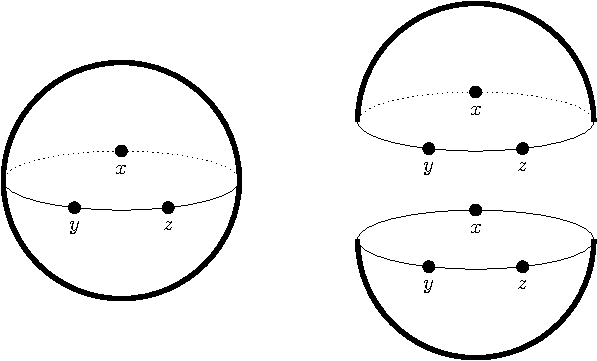
\includegraphics[width= 0.85\linewidth]{H8}
				\caption{\small\textit{\color{lichsutoanhoc}Hình $8$: Xoắn ốc Theodorus.}}
				\vspace*{-10pt}
			\end{figure}
		Plato có vai trò quan trọng trong lịch sử toán học phần lớn vì ông là người truyền cảm hứng và là người sáng lập Học viện đào tạo ra nhiều nhà toán học, cũng như do sự nhạy bén của ông về sự phân biệt ở Hy Lạp cổ đại giữa số học (theo nghĩa của lý thuyết về các con số) và kỹ thuật tính toán. 
		\vskip 0.1cm
		Plato cho rằng toán học là cần thiết cho doanh nhân và quân sự, ``phải học nghệ thuật của những con số, nếu không anh ta sẽ không biết cách dàn quân".
		\vskip 0.1cm
		Mặt khác, nhà triết học phải là một nhà số học ``bởi vì anh ta phải nhảy ra khỏi biển của những thay đổi và nắm giữ bản thể đích thực." Hơn nữa, Plato nói trong tác phẩm \textit{Cộng hòa (The Republic)}: ``Số học có tác dụng rất lớn và nâng cao, buộc tâm trí nghĩ về số trừu tượng."
		\vskip 0.1cm 
		Trong số học, Plato đã nhìn thấy một hố ngăn cách lý thuyết và các khía cạnh tính toán, cũng như trong hình học, ông cũng tán thành toán học thuần túy chống lại quan điểm duy vật.  
		\vskip 0.1cm
		Bất kỳ một trong số vô số đường kính của đường tròn là trục đối xứng của hình. Bất cứ điểm nào trên một đường thẳng kéo dài vô hạn có thể được coi là tâm của đối xứng, giống như bất kỳ đường thẳng nào vuông góc với đường thẳng đã cho là trục đối xứng của đường thẳng đã cho. Triết học Plato, với sự áp dụng các ý tưởng của nó, tự nhiên sẽ tìm thấy vai trò của đường thẳng và đường tròn giữa các hình hình học. Tương tự, Plato tôn vinh tam giác.
		\vskip 0.1cm 
		Sự liên kết của bốn khối đa diện đầu tiên với bốn yếu tố phổ quát truyền thống của vũ trụ đã cung cấp cho Plato trong \textit{Timaeus}  một lý thuyết thống nhất tuyệt đẹp về vật chất, theo đó mọi thứ đều được xây dựng bằng các tam giác vuông lý tưởng. Toàn bộ sinh lý học, cũng như khoa học về chất trơ, dựa trên các hình tam giác.
		\vskip 0.1cm
		Pythagoras nổi tiếng là người đã thiết lập toán học như một chủ đề tự do, nhưng Plato đã có ảnh hưởng trong việc làm cho toán học trở thành một phần thiết yếu của chương trình đào tạo.
		\vskip 0.1cm
		Có lẽ bị ảnh hưởng bởi Archytas, Plato đã thêm vào các chủ đề ban đầu trong bộ bốn (quadrivium: Số học, Hình học, Âm nhạc, Thiên văn) một môn học mới: Hình học không gian, vì ông tin rằng hình học không gian đã không được nhấn mạnh đầy đủ. Plato cũng thảo luận về nền tảng của toán học, làm rõ một số định nghĩa và xây dựng lại các giả thiết. Ông nhấn mạnh rằng lý luận được sử dụng trong hình học không đề cập đến những con số hữu hình mô tả chúng, mà là những ý tưởng tuyệt đối mà chúng đại diện. 
		\vskip 0.1cm
		Những người theo thuyết Pythagoras đã định nghĩa điểm là ``sự thống nhất có vị trí," nhưng Plato lại nghĩ về nó như là sự khởi đầu của một đường thẳng.
		\vskip 0.1cm 
		Định nghĩa của một đường là ``chiều dài không có chiều rộng" dường như bắt nguồn từ trường phái Plato.
		\vskip 0.1cm
		Trong số học, Plato không chỉ nhấn mạnh sự phân biệt giữa số lẻ và số chẵn, mà còn là các loại ``chẵn nhân chẵn", ``chẵn nhân lẻ" và ``lẻ nhân lẻ". Mặc dù ta biết rằng Plato đã thêm vào các tiên đề của toán học, chúng ta không có một cơ sở nào để khẳng định điều này.
		\vskip 0.1cm
		Rất ít đóng góp toán học cụ thể được quy cho Plato. Một công thức cho bộ ba Pythagoras -- ${(2n)^2} + {({n^2} - 1)^2} = {({n^2} + 1)^2}$, trong đó  $n$ là số tự nhiên bất kỳ -- mang tên Plato, nhưng đây chỉ là một phiên bản sửa đổi của kết quả được người Babylon và người Pythagoras đã biết. 
		\vskip 0.1cm
		Có lẽ thực sự có ý nghĩa quan trọng hơn cả trong những thứ được gán cho Plato là cái gọi là phương pháp phân tích (analytic method).
		\vskip 0.1cm
		Trong chứng minh toán học, ta bắt đầu với những gì đã cho, và từ các tiên đề và các định đề. Tiến hành từng bước một, sau đó đến khẳng định cần được chứng minh.
		\vskip 0.1cm
		Plato dường như đã chỉ ra rằng  về mặt sư phạm, khi không tìm được một chuỗi lý luận hiển nhiên từ giả thiết đến kết luận, thường là thuận tiện hơn nếu ta bắt đầu bằng mệnh đề cần được chứng minh và từ đó suy ra một kết luận được biết là đúng. Nếu, sau đó, có thể đảo ngược các bước trong chuỗi lý luận này, kết quả sẽ là mệnh đề đã được chứng minh.
		\vskip 0.1cm
		Plato không hẳn là người đầu tiên nêu lên quan điểm phân tích.  Nhưng những gì Plato có thể đã làm là chính thức hóa quá trình này, hoặc có thể ông đã đặt tên cho nó.
		\vskip 0.1cm
		Vai trò của Plato trong lịch sử toán học vẫn còn bị tranh cãi gay gắt. Một số người coi ông là một nhà tư tưởng đặc biệt sâu sắc và nhạy bén. Những người khác hình dung ông như một người đã thu hút các nhà toán học theo con đường lý luận trừu tượng, đi xa những vấn đề thực tiễn. 
		\vskip 0.1cm
		Trong mọi trường hợp, ít ai có thể phủ nhận rằng Plato đã có tác động to lớn đối với sự phát triển của toán học. Học viện Plato ở Athens trở thành trung tâm toán học của thế giới, và từ ngôi trường này, xuất hiện các giáo viên và nghiên cứu viên hàng đầu đến vào giữa thế kỷ thứ tư TCN. Trong số này, nổi tiếng nhất là Eudoxus xứ Cnidus (khoảng $408-335$ TCN),  một học trò của Plato và người đã trở thành nhà toán học và nhà thiên văn học nổi tiếng nhất trong thời đại của mình.
		\vskip 0.1cm
		\textbf{\color{lichsutoanhoc}Tài liệu chính dùng để soạn}
		\vskip 0.1cm
		[$1$] David M. Burton, \textit{The History of Mathematics, An Introduction}, Seventh Edition, McGraw--Hill, $2011$. Chapter $3$: The Beginnings of Greek Mathematics, pp. $116-139$.
		\vskip 0.1cm
		[$2$] Euclid’s \textit{Elements of Geometry}, edited and provided with a modern English translation by Richard Fitzpatrick, Independently published, $2008$, $544$ p.
		\vskip 0.1cm
		[$3$] David Fowler, \textit{The Mathematics of Plato’s Academy}, Second Edition, Clarendon Press, Oxford, $1999$, $441$ p.
		\vskip 0.1cm   
		[$4$] Thomas Heath, \textit{A History of Greek Mathematics}, Oxford at the Clarendon Press, $1921$, Volume $1$: From Thales to Euclid, pp. $170-315$.
		\vskip 0.1cm   
		[$5$] Victor J. Katz, \textit{A History of Mathematics, An Introduction}, Third Edition, Addison--Wesley, $2009$. Chapter $2$: \textit{The Beginnings of Mathematics in Greek}, pp. $40-49$.
		\vskip 0.1cm
		[$6$] Uta C. Merzbach and Carl B. Boyer, \textit{A
			History of Mathematics}, Third Edition, John Wiley \& Sons, $2011$, pp. $65-80$.
		\vskip 0.1cm
		[$7$] George Johston Allman, \textit{Greek Geometry, From Thales to Euclid}, Dublin Universty Press, $1885$, $432$ p.
		\vskip 0.1cm  
		[$8$] R. Lloyd, \textit{Early Greek Science: Thales to Aristotle}, $1970$, Chatto \& Windus, London, $156$ p.
		\vskip 0.1cm 
		[$9$] Arpad Szabo, \textit{The beginnings of Greek Mathematics}, Springer, $1978$, $363$ p.
\end{multicols}